\que{Задача об аэродинамическом нагреве.}

\begin{figure}[H]
  \centering
  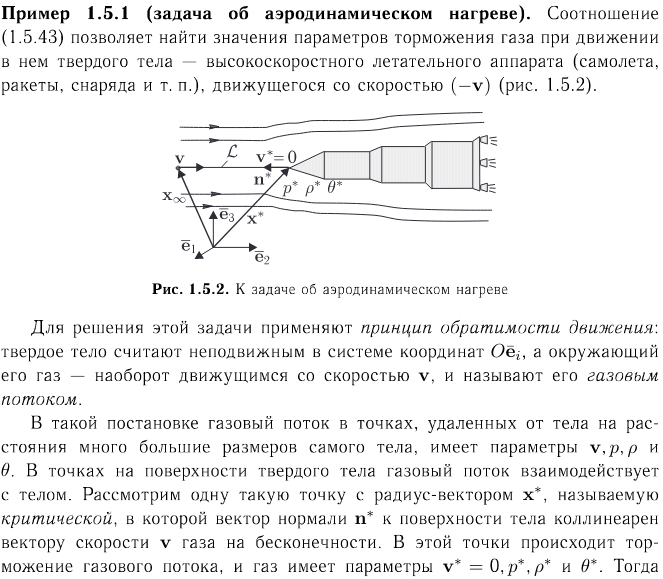
\includegraphics[width=0.7\linewidth]{img/50_01.png}
\end{figure}
\begin{figure}[H]
  \centering
  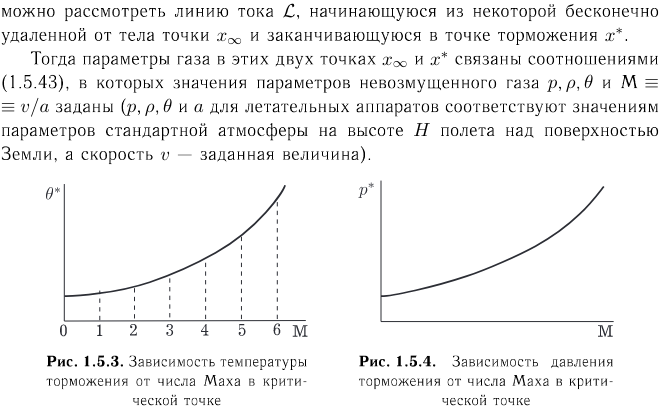
\includegraphics[width=0.7\linewidth]{img/50_02.png}
\end{figure}

Упомянутые соотношения (1.5.43):
\begin{align*}
  \dfrac{p}{p^*} &= \left( 1 + \dfrac{k-1}{2} M^2 \right)^{- k / (k-1)}, \\
  \dfrac{\rho}{\rho^*} &= \left( 1 + \dfrac{k-1}{2} M^2 \right)^{-1 / (k-1)}, \\
  \dfrac{\theta}{\theta^*} &= \left( 1 + \dfrac{k-1}{2} M^2 \right)^{-1}.
\end{align*}
